%
% $Id: blank.tex,v 2.0 2010-01-05 18:50:50+09 kobayasi Exp $
%
% Mar 21, 2001:  Revision Control Started!!
%
\documentclass[11pt]{jreport}
\usepackage{newcent}             % PDFへの変換後の品質を高める
\usepackage[dvipdfmx]{graphicx}
\usepackage{color}
\definecolor{purple}{rgb}{0.6,0,0.4}
\definecolor{brown}{cmyk}{0,0.81,1,0.60}
\usepackage{listings, jlisting}
\renewcommand{\lstlistingname}{ソース}
\lstset
{
breaklines = true,
language=Java,
keywordstyle={\color{purple}},
commentstyle={\color{brown}},
numbers=left,
frame=single,
tabsize=4
}


%
%\usepackage[doctor]{gaiyo}      % 博士論文要旨の場合
%\usepackage[master]{gaiyo}      % 修士論文要旨の場合
\usepackage{sotsuron}               % 卒業研究概要の場合
% \usepackage[junior]{gaiyo}      % 専門演習レポートの場合

\setlength\textfloatsep{0pt}

\title{\bfseries スマートフォンのモーションセンサを利用した\\個人認証アプリケーションの開発}
\author{情11-0170 高坂 賢佑}
\date{}
\renewcommand{\bibname}{参考文献,参考URL等}

\begin{document}
\maketitle

\tableofcontents
\listoffigures

\chapter*{はじめに}
スマートフォンが徐々に普及しつつある現在,スマートフォンの個人認証方法は画面上に表示される
ソフトウェアキーボードのテンキーを用いたパスコード認証が大部分を占めている.しかし,この認証方法は
,画面ロックを解除するたびに画面に表示されたソフトウェアキーボードを目で見て指でタッチして操作する
必要が有るため,ユーザにとって煩雑な作業である.また,パスコード認証では,あらかじめ決められた文字種の
中から1つずつ選択したものを元にパスコードを構築していくという性質上,パターン数は限られ,自由度は
限定されてしまう.そこで,パスコード認証が抱える,認証の煩雑さを解消し,かつ,自由度が高くより直感的に
個人認証を行えるアプリケーションを開発する.このアプリケーションには,一般的なスマートフォンに
搭載されている加速度センサとジャイロセンサを用いることとする.

\chapter{使用するセンサについて}
	\section{加速度センサ}
	加速度センサとは,X軸,Y軸,Z軸の基準軸に対して直線運動の加速度をそれぞれ検出し,値として取り出すこと
	のできるセンサである.ここでいう加速度とは,端末における,単位時間あたりの速度の変化率のことを指し,
	図\ref{sensor}における直線で示した矢印の方向が正の値,逆が負の値をとる.
	
	\section{ジャイロセンサ}
	ジャイロセンサとは,X軸,Y軸,Z軸の基準軸に対して回転運動の角速度をそれぞれ検出し,値として取り出す
	ことのできるセンサである.ここでいう角速度とは,端末における,単位時間あたりの回転角のことを指し,
	右ねじを回した時に,図\ref{sensor}における直線で示した矢印の方向に進むような橙色で示した回転が正,
    逆が負の値をとる.

    % センサのイメージ図
    \begin{figure}[htbp]
      \begin{center}
        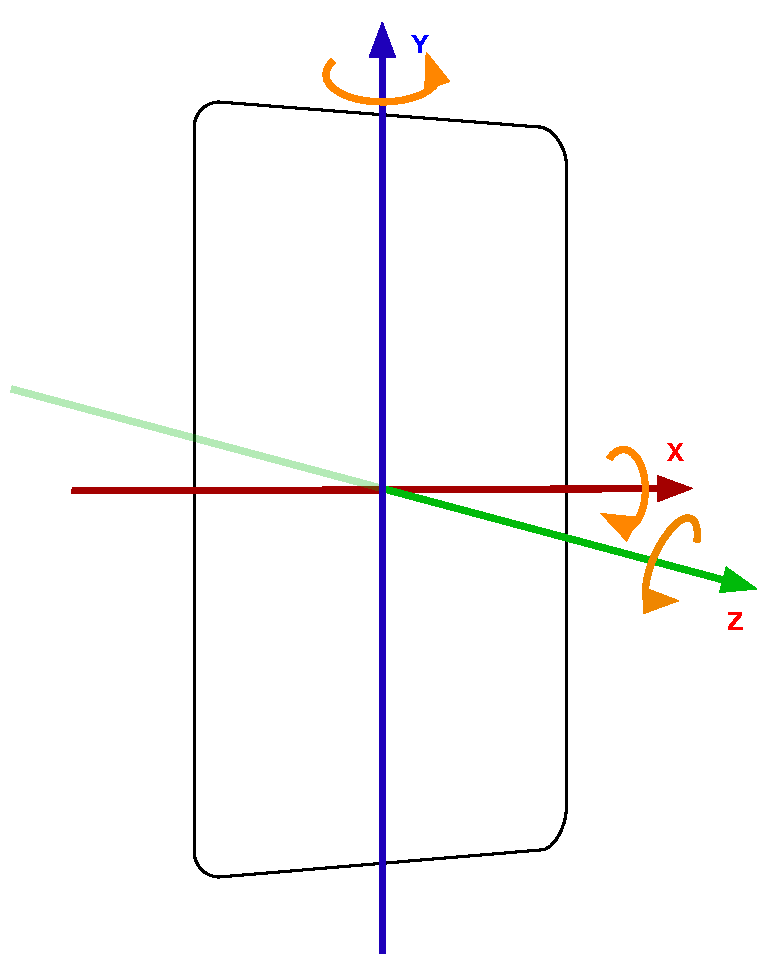
\includegraphics[width=7cm, bb=0 0 373 469]{SmartphoneSensor.pdf}
        \caption{モーションセンサの座標系イメージ}
        \label{sensor}
      \end{center}
    \end{figure}

\chapter{先行研究}
	\section{坂本の研究}
	坂本の研究では,ユーザが入力したモーションの数値化に加速度センサを用い,あらかじめ保存しておいた
    複数のジェスチャパターンのデータと認証時に入力したデータをパターンマッチング方式のアルゴリズムを用いて
    比較することで個人認証を行った.

    しかし,このプログラムは扱うジェスチャによって認証率が高いものと低いものの二分化の傾向が見られるという問題点
    があった.
	\section{兎澤の研究}
    兎澤の研究では,モーションの数値化に加速度センサとジャイロセンサを用い,認証システムの中核に相関関数を
    用いたシステムを開発し,ユーザに三回入力させたモーションの平均値データと認証時に入力したデータの類似性を
    調べることで個人認証を行った.これにより,坂本の研究で指摘されていた成功率の二分化や,立体的な動きへの
    対応を可能にし,モーションの対応幅を広げることができた.

    しかし,全体的な認証成功率が低く,特に手首のスナップを用いるような動きの小さいモーションに対して認証率が
    特に低く出るなど,対応できるモーションに限りがあるという問題点が指摘されていた.

\chapter{本研究のシステム}
	\section{本研究の概要}
	本研究では,兎澤の研究で挙げられていた,全体的な認証成功率の低さや対応できるモーションに限りがあるという点を
    改善することを目標とする.具体的には,より幅広いモーション,特に手首のスナップを用いるような比較的動きの小さい
    モーションに対しての,個人認証の全体的な認証成功率の向上を目指し,より実用レベルに近いアプリケーションの開発を
    行う.
	\section{システムの概要}
	本研究では,先行研究をもとにAndroidデバイス上で動作するアプリケーションとしてシステムを構築する.システムの
    動作フローを図hogeに示す.\textcolor{red}{システム動作フロー図を挿入する}

    ユーザはまず,新規登録モードにおいて個人認証に用いる鍵情報となるモーションを登録する.新規登録モードでは
    ユーザに同一のモーションを三回入力させ,入力した三回のモーションが同一のモーションであると確認できた場合に
    そのモーションの平均値をユーザのモーションデータとして登録する.
    個人認証時には,事前に新規登録モードにおいてモーションデータを登録しておいたユーザ名を入力させ,該当ユーザが
    登録されていると確認できた場合にのみ,ユーザにモーションを一回入力させる.入力されたモーションデータと
    指定したユーザ名で登録されたモーションデータ間の相関を取ることで個人認証を行う.
    また,新規登録モードにおいて登録したユーザ名および登録データに関しては,データ閲覧モードにおいて閲覧することが
    可能である.
	\section{新規登録モード}
    \textcolor{red}{画面のサンプル図を挿入する}
	新規登録モードでは,ユーザに登録するユーザ名を入力させた後に同一のモーションを三回入力させる.
    モーション入力ボタンを押した後に三秒間のインターバルを挟み,その後の三秒間で0.03秒ごとに加速度センサ
    およびジャイロセンサよりデータを取得する.この際,一秒ごとに端末にバイブレーションを発生させることで,
    ユーザが視覚に頼らずとも経過時間が把握できるようにしている.
    三回分のデータの取得が完了した段階で,まずは入力されたモーションが比較的大きなモーションなのか,小さいモーション
    なのかを判断する.ここで小さいモーションであると判断されれば,データの増幅処理を行う.この処理を行うことにより,
    先行研究において指摘されていた,動きの小さいモーションにおいて個人認証の成功率が低くなるという課題の対策をしている.
    データの増幅処理を行った後,次はデータに対して高速フーリエ変換を用いたローパスフィルタ処理を行う.そして
    加速度データやジャイロデータをそれぞれ距離データ,角度データに変換し,三回分のデータそれぞれが同一のモーションであるかの
    確認を行う.ここで同一のモーションではあるが,モーションデータに取得回数ごとに発生しうる時間的なモーションのズレが見られた
   場合は,このズレを修正する.修正が完了すれば,これら三回分のデータの平均値を取り,これを個人認証時の鍵情報として登録する.
	\section{認証試験モード}
    \textcolor{red}{画面のサンプル図を挿入する}
	認証試験モードでは,新規登録モードにて事前に登録おいたユーザ名を入力させ,そのユーザが登録されていることを確認した後に
    ユーザにモーションを一回入力させる.こちらも新規登録モードと同じく,モーション入力ボタンを落ちた後に三秒間のインターバルを挟み,
    その後の三秒間で0.03秒ごとに加速度センサおよびジャイロセンサよりデータを取得する.この際,一秒ごとに端末にバイブレーションを発生
    させる.
    認証試験モードではユーザがモーションを入力するのは一回のみとなる.入力した後,まずは指定したユーザ名をもとに新規登録モード
    にて登録したモーションデータを読み出す.保存データには鍵情報の他に登録時にデータを増幅したかどうかのフラグ情報もあるため,これを
    もとに先ほどユーザに入力させたモーションのデータに増幅をかけるかどうかを判断する.
    この処理が終われば,次に高速フーリエ変換を用いたローパスフィルタ処理を行い,加速度データやジャイロデータをそれぞれ距離データ,角度データ
    に変換する.そして新規登録モードにて登録したデータと今回ユーザが入力したデータ間の相関をとり,個人認証を行う.
	\section{登録データ一覧モード}
    \textcolor{red}{モードの名称を統一する}
    \textcolor{red}{画面のサンプル図を挿入する}
	登録データ一覧モードでは,新規登録モードにて登録されたユーザ名を一覧で見ることが出来る.また,その中からユーザ名を選択すると
    そのユーザが登録したモーションデータを見ることが出来る.
\chapter{実験と考察}
	\section{実験方法}
	今回開発したシステムを用いて,以下に挙げるそれぞれのモーションを新規登録モードにてあらかじめ登録しておき,
    認証試験モードにて個人認証の成功率を検証する.認証はそれぞれのモーションにつき十回ずつ行い,この結果から
    個人認証の成功率を算出する.
	\section{実験結果}
	\textcolor{red}{実験結果を表を用いて示す}
	\section{考察}
    \textcolor{red}{実験結果に対する考察}
	\section{課題}
	\textcolor{red}{実験結果より生じた課題}
\chapter{おわりに}


\chapter*{謝辞}
本研究のプログラム開発や実験,本論文の執筆にあたり,手厚い指導と様々な助言をしていただいた,関西大学総合情報学部セキュア情報システム研究室の
小林孝史准教授に深く感謝いたします.また,研究テーマの選定をはじめ,日頃から有益なアドバイスを頂いた同研究室の皆様に感謝いたします.

\end{document}
